\documentclass[]{article}
\usepackage{lmodern}
\usepackage{amssymb,amsmath}
\usepackage{ifxetex,ifluatex}
\usepackage{fixltx2e} % provides \textsubscript
\ifnum 0\ifxetex 1\fi\ifluatex 1\fi=0 % if pdftex
  \usepackage[T1]{fontenc}
  \usepackage[utf8]{inputenc}
\else % if luatex or xelatex
  \ifxetex
    \usepackage{mathspec}
  \else
    \usepackage{fontspec}
  \fi
  \defaultfontfeatures{Ligatures=TeX,Scale=MatchLowercase}
\fi
% use upquote if available, for straight quotes in verbatim environments
\IfFileExists{upquote.sty}{\usepackage{upquote}}{}
% use microtype if available
\IfFileExists{microtype.sty}{%
\usepackage{microtype}
\UseMicrotypeSet[protrusion]{basicmath} % disable protrusion for tt fonts
}{}
\usepackage[margin=1in]{geometry}
\usepackage{hyperref}
\hypersetup{unicode=true,
            pdftitle={Elections},
            pdfauthor={Taha},
            pdfborder={0 0 0},
            breaklinks=true}
\urlstyle{same}  % don't use monospace font for urls
\usepackage{color}
\usepackage{fancyvrb}
\newcommand{\VerbBar}{|}
\newcommand{\VERB}{\Verb[commandchars=\\\{\}]}
\DefineVerbatimEnvironment{Highlighting}{Verbatim}{commandchars=\\\{\}}
% Add ',fontsize=\small' for more characters per line
\usepackage{framed}
\definecolor{shadecolor}{RGB}{248,248,248}
\newenvironment{Shaded}{\begin{snugshade}}{\end{snugshade}}
\newcommand{\KeywordTok}[1]{\textcolor[rgb]{0.13,0.29,0.53}{\textbf{#1}}}
\newcommand{\DataTypeTok}[1]{\textcolor[rgb]{0.13,0.29,0.53}{#1}}
\newcommand{\DecValTok}[1]{\textcolor[rgb]{0.00,0.00,0.81}{#1}}
\newcommand{\BaseNTok}[1]{\textcolor[rgb]{0.00,0.00,0.81}{#1}}
\newcommand{\FloatTok}[1]{\textcolor[rgb]{0.00,0.00,0.81}{#1}}
\newcommand{\ConstantTok}[1]{\textcolor[rgb]{0.00,0.00,0.00}{#1}}
\newcommand{\CharTok}[1]{\textcolor[rgb]{0.31,0.60,0.02}{#1}}
\newcommand{\SpecialCharTok}[1]{\textcolor[rgb]{0.00,0.00,0.00}{#1}}
\newcommand{\StringTok}[1]{\textcolor[rgb]{0.31,0.60,0.02}{#1}}
\newcommand{\VerbatimStringTok}[1]{\textcolor[rgb]{0.31,0.60,0.02}{#1}}
\newcommand{\SpecialStringTok}[1]{\textcolor[rgb]{0.31,0.60,0.02}{#1}}
\newcommand{\ImportTok}[1]{#1}
\newcommand{\CommentTok}[1]{\textcolor[rgb]{0.56,0.35,0.01}{\textit{#1}}}
\newcommand{\DocumentationTok}[1]{\textcolor[rgb]{0.56,0.35,0.01}{\textbf{\textit{#1}}}}
\newcommand{\AnnotationTok}[1]{\textcolor[rgb]{0.56,0.35,0.01}{\textbf{\textit{#1}}}}
\newcommand{\CommentVarTok}[1]{\textcolor[rgb]{0.56,0.35,0.01}{\textbf{\textit{#1}}}}
\newcommand{\OtherTok}[1]{\textcolor[rgb]{0.56,0.35,0.01}{#1}}
\newcommand{\FunctionTok}[1]{\textcolor[rgb]{0.00,0.00,0.00}{#1}}
\newcommand{\VariableTok}[1]{\textcolor[rgb]{0.00,0.00,0.00}{#1}}
\newcommand{\ControlFlowTok}[1]{\textcolor[rgb]{0.13,0.29,0.53}{\textbf{#1}}}
\newcommand{\OperatorTok}[1]{\textcolor[rgb]{0.81,0.36,0.00}{\textbf{#1}}}
\newcommand{\BuiltInTok}[1]{#1}
\newcommand{\ExtensionTok}[1]{#1}
\newcommand{\PreprocessorTok}[1]{\textcolor[rgb]{0.56,0.35,0.01}{\textit{#1}}}
\newcommand{\AttributeTok}[1]{\textcolor[rgb]{0.77,0.63,0.00}{#1}}
\newcommand{\RegionMarkerTok}[1]{#1}
\newcommand{\InformationTok}[1]{\textcolor[rgb]{0.56,0.35,0.01}{\textbf{\textit{#1}}}}
\newcommand{\WarningTok}[1]{\textcolor[rgb]{0.56,0.35,0.01}{\textbf{\textit{#1}}}}
\newcommand{\AlertTok}[1]{\textcolor[rgb]{0.94,0.16,0.16}{#1}}
\newcommand{\ErrorTok}[1]{\textcolor[rgb]{0.64,0.00,0.00}{\textbf{#1}}}
\newcommand{\NormalTok}[1]{#1}
\usepackage{graphicx,grffile}
\makeatletter
\def\maxwidth{\ifdim\Gin@nat@width>\linewidth\linewidth\else\Gin@nat@width\fi}
\def\maxheight{\ifdim\Gin@nat@height>\textheight\textheight\else\Gin@nat@height\fi}
\makeatother
% Scale images if necessary, so that they will not overflow the page
% margins by default, and it is still possible to overwrite the defaults
% using explicit options in \includegraphics[width, height, ...]{}
\setkeys{Gin}{width=\maxwidth,height=\maxheight,keepaspectratio}
\IfFileExists{parskip.sty}{%
\usepackage{parskip}
}{% else
\setlength{\parindent}{0pt}
\setlength{\parskip}{6pt plus 2pt minus 1pt}
}
\setlength{\emergencystretch}{3em}  % prevent overfull lines
\providecommand{\tightlist}{%
  \setlength{\itemsep}{0pt}\setlength{\parskip}{0pt}}
\setcounter{secnumdepth}{0}
% Redefines (sub)paragraphs to behave more like sections
\ifx\paragraph\undefined\else
\let\oldparagraph\paragraph
\renewcommand{\paragraph}[1]{\oldparagraph{#1}\mbox{}}
\fi
\ifx\subparagraph\undefined\else
\let\oldsubparagraph\subparagraph
\renewcommand{\subparagraph}[1]{\oldsubparagraph{#1}\mbox{}}
\fi

%%% Use protect on footnotes to avoid problems with footnotes in titles
\let\rmarkdownfootnote\footnote%
\def\footnote{\protect\rmarkdownfootnote}

%%% Change title format to be more compact
\usepackage{titling}

% Create subtitle command for use in maketitle
\newcommand{\subtitle}[1]{
  \posttitle{
    \begin{center}\large#1\end{center}
    }
}

\setlength{\droptitle}{-2em}
  \title{Elections}
  \pretitle{\vspace{\droptitle}\centering\huge}
  \posttitle{\par}
  \author{Taha}
  \preauthor{\centering\large\emph}
  \postauthor{\par}
  \predate{\centering\large\emph}
  \postdate{\par}
  \date{6/1/2018}


\begin{document}
\maketitle

\subsection{Introduction}\label{introduction}

This is a fun big data anaytics project that seeks to uses sentiment
analysis to analyse the popularity of political figures in Pakistan.
Before we go into the analytics, let us get a bit of a background on the
upcoming Pakistani elections.

\subsubsection{Background}\label{background}

Pakistan is a parliamentary democratic republic with a bicameral
legislature. Every five years the federal National Assembly alongside
the provinical assemblies hold elections. Historically, a number of
political parties have contested these elections but in recent times the
most popular ones have been Pakistan Muslim League Nawaz (PMLN),
Pakistan Tehrik-e-Insaf (PTI) and Pakistan People's Party (PPP). All
three parties have their strongholds in different provinces of the
country and contest elections for the national assembly every five
years. The party with current majority in the National Assembly is PMLN
while regionally PMLN, PTI and PPP have majorities in the Punjab, KPK
and Sindh provincial assemblies.
\includegraphics{https://simplemaps.com/static/svg/pk/pk.svg}

For the upcoming elections, all three parties have nominated a candidate
for the post of the Prime Minister of Pakistan. The ex-cricketer turned
politician Imran Khan is PTI's candidate, ex-Prime Minister's brother
and popular Chief Minister of Punjab, Shehbaz Sharif is PMLN's nominee
while PPP is backing their Chairman, the son and grandson of ex-Prime
Ministers, Bilawal Bhutto.

\includegraphics[width=0.33\linewidth]{https://timesofindia.indiatimes.com/thumb/msid-63286527,width-400,resizemode-4/63286527}
\includegraphics[width=0.33\linewidth]{https://timesofindia.indiatimes.com/thumb/msid-62438429,width-400,resizemode-4/62438429}
\includegraphics[width=0.33\linewidth]{https://timesofislamabad.com/digital_images/medium/2017-04-04/bilawal-bhutto-lashes-out-at-pml-n-1513928280-5884}

\subsection{Getting the Data}\label{getting-the-data}

I gathered the required data from Twitter through the package
\texttt{twitteR}. Note that there are other packages that would have
worked- \texttt{rtweet} is another good one- but this one seems to do
the job well enough.

We begin by gathering the last 1500 tweets that have mentioned Imran
Khan, Shehbaz Sharif and Bilawal Bhutto. A \texttt{getFeed()} creates a
list of tweets for a given string and extracts the text from them.
Applying it to our vector of candidates gives us the required twitter
feeds for them.

\begin{Shaded}
\begin{Highlighting}[]
\NormalTok{candidates <-}\StringTok{ }\KeywordTok{c}\NormalTok{(}\StringTok{"Imran Khan"}\NormalTok{, }\StringTok{"Shehbaz Sharif"}\NormalTok{, }\StringTok{"Bilawal Bhutto"}\NormalTok{)}

\NormalTok{getFeed <-}\StringTok{ }\ControlFlowTok{function}\NormalTok{(candidate)\{}
\NormalTok{  tweets<-}\StringTok{ }\KeywordTok{searchTwitter}\NormalTok{(candidate, }\DataTypeTok{n=}\DecValTok{1500}\NormalTok{)}
\NormalTok{  feed<-}\StringTok{ }\KeywordTok{lapply}\NormalTok{(tweets, }\ControlFlowTok{function}\NormalTok{(x)\{x}\OperatorTok{$}\KeywordTok{getText}\NormalTok{()\})}
  \KeywordTok{return}\NormalTok{(feed)}
\NormalTok{\}}

\NormalTok{candidates_feeds<-}\StringTok{ }\KeywordTok{sapply}\NormalTok{(candidates, getFeed)}
\end{Highlighting}
\end{Shaded}

Let us check a tweet to see if we are on the right track.

\begin{Shaded}
\begin{Highlighting}[]
\NormalTok{feed_IK <-}\StringTok{ }\NormalTok{candidates_feeds[,}\StringTok{"Imran Khan"}\NormalTok{]}
\NormalTok{feed_IK[}\DecValTok{150}\NormalTok{]}
\end{Highlighting}
\end{Shaded}

\begin{verbatim}
## [[1]]
## [1] "RT @PTIofficial: Chairman PTI Imran Khan Exclusive Interview on BBC News HARDtalk with Zeinab Badawi (04.06.18) 8/12\n#IKonBBC @ImranKhanPTI…"
\end{verbatim}

Sounds about right. Now we can break down these tweets into individual
words that we can then manipulate. A \texttt{getWords()} function that
splits the strings along spaces will be a good way. Let's get all the
words in tweets about Imran Khan using it.

\begin{Shaded}
\begin{Highlighting}[]
\NormalTok{getWords<-}\StringTok{ }\ControlFlowTok{function}\NormalTok{(candidate)\{}
\NormalTok{  feed <-}\StringTok{ }\NormalTok{candidates_feeds[,candidate]}
\NormalTok{  wordList <-}\StringTok{ }\KeywordTok{str_split}\NormalTok{(feed, }\StringTok{' '}\NormalTok{)}
\NormalTok{  wordList <-}\StringTok{ }\KeywordTok{unlist}\NormalTok{(wordList)}
  \KeywordTok{return}\NormalTok{(wordList)}
\NormalTok{\}}

\NormalTok{words_IK <-}\StringTok{ }\KeywordTok{getWords}\NormalTok{(}\StringTok{"Imran Khan"}\NormalTok{)}
\end{Highlighting}
\end{Shaded}

Now you must be, rightly, wondering if we need to clean up this data. We
do. Let's have a look at the most repeated words used in tweets related
to Imran Khan.

\begin{Shaded}
\begin{Highlighting}[]
\KeywordTok{head}\NormalTok{(}\KeywordTok{sort}\NormalTok{(}\KeywordTok{table}\NormalTok{(words_IK), }\DataTypeTok{decreasing =} \OtherTok{TRUE}\NormalTok{))}
\end{Highlighting}
\end{Shaded}

\begin{verbatim}
## words_IK
##    RT Imran  Khan    on   the  with 
##  1166  1039   925   420   397   397
\end{verbatim}

As we can see the most repeated words are Imran Khan's name, `RT' for
retweet and a few commonly used stop words. These are not very
insightful and should be removed before any analysis. In addition let us
look at a random range of words in the vector.

\begin{Shaded}
\begin{Highlighting}[]
\KeywordTok{sort}\NormalTok{(}\KeywordTok{table}\NormalTok{(words_IK), }\DataTypeTok{decreasing =} \OtherTok{TRUE}\NormalTok{)[}\DecValTok{100}\OperatorTok{:}\DecValTok{120}\NormalTok{]}
\end{Highlighting}
\end{Shaded}

\begin{verbatim}
## words_IK
##               or          started             have             him. 
##               48               47               46               46 
##            house           kicked           rushed        troubling 
##               46               46               46               46 
##             کتاب @MaleehaHashmey:       convincing             been 
##               46               45               45               43 
##              she           Abbasi               be          because 
##               41               40               39               39 
##    @ImranKhanPTI               If               ko               do 
##               38               38               38               37 
##      @RehamKhan1 
##               36
\end{verbatim}

We can see that the data is infested with punctuation marks, numbers,
hastags, etc. Some tweets are in Urdu, Punjabi and other regional
scripts which can not be process. In addition, the words are case
sensitive as of now which is highly unnecessary. Finally there must be a
lot of words smaller than 3 characters that will probably not be very
insightful. We need to rid the data of all these. Thus, we need to
modify our \texttt{getWords()} function.

\begin{Shaded}
\begin{Highlighting}[]
\NormalTok{getWords <-}\StringTok{ }\ControlFlowTok{function}\NormalTok{(candidate)\{}
\NormalTok{  feed <-}\StringTok{ }\NormalTok{candidates_feeds[,candidate]}
\NormalTok{  words <-}\StringTok{ }\KeywordTok{str_split}\NormalTok{(feed, }\StringTok{' '}\NormalTok{)}
\NormalTok{  words <-}\StringTok{ }\KeywordTok{unlist}\NormalTok{(words)}
\NormalTok{  words <-}\StringTok{ }\KeywordTok{sub}\NormalTok{(}\StringTok{"^*[[:punct:]]"}\NormalTok{, }\StringTok{""}\NormalTok{, words)}
\NormalTok{  words <-}\StringTok{ }\KeywordTok{sub}\NormalTok{(}\StringTok{"[[:punct:]]*$"}\NormalTok{, }\StringTok{""}\NormalTok{, words)}
  \CommentTok{# Remove Urdu words}
\NormalTok{  removeIdx <-}\StringTok{ }\KeywordTok{which}\NormalTok{(}\KeywordTok{grepl}\NormalTok{(}\StringTok{"[^A-Za-z]"}\NormalTok{, words))}
  \ControlFlowTok{if}\NormalTok{ (}\KeywordTok{length}\NormalTok{(removeIdx) }\OperatorTok{>}\StringTok{ }\DecValTok{0}\NormalTok{)\{}
\NormalTok{    words <-}\StringTok{ }\NormalTok{words[}\OperatorTok{-}\NormalTok{removeIdx]  }
\NormalTok{  \}}
  \CommentTok{# Make lower caps}
\NormalTok{  words <-}\StringTok{ }\KeywordTok{tolower}\NormalTok{(words)}
  \CommentTok{# Remove candidate name, stop words and empty strings.}
\NormalTok{  candidateName <-}\StringTok{ }\KeywordTok{tolower}\NormalTok{(}\KeywordTok{unlist}\NormalTok{(}\KeywordTok{strsplit}\NormalTok{(candidate, }\DataTypeTok{split =} \StringTok{" "}\NormalTok{)))}
\NormalTok{  wordsToRemove <-}\StringTok{ }\KeywordTok{c}\NormalTok{(}\KeywordTok{stopwords}\NormalTok{(), candidateName, }\StringTok{"RT"}\NormalTok{)}
\NormalTok{  words <-}\StringTok{ }\NormalTok{words[}\OperatorTok{!}\NormalTok{(words }\OperatorTok\StringTok{ }\NormalTok{wordsToRemove) }\OperatorTok{&}\StringTok{ }\NormalTok{(words }\OperatorTok{!=}\StringTok{ ""}\NormalTok{) }\OperatorTok{&}\StringTok{ }\KeywordTok{nchar}\NormalTok{(words)}\OperatorTok{>}\DecValTok{2}\NormalTok{]}
  
  \KeywordTok{return}\NormalTok{(words)}
\NormalTok{\}}
\end{Highlighting}
\end{Shaded}

Now we should have clean data to begin our analyses. We can firstly
begin by visualizing what were the most used words for these candidates.
One way to do that is through a world cloud of the output of our
\texttt{getWords()} function.
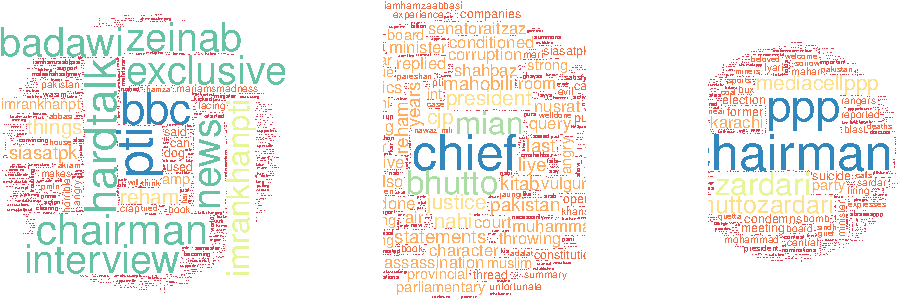
\includegraphics{Elections_files/figure-latex/makeWordCloud function-1.pdf}


\end{document}
